\section{Results}

\subsection{Integrative-microbiomics, a webtool}

To motivate and enable; researchers and clinicians to opt for an integrative strategy when analysing multi biome datasets, we developed a web tool “Integrative Microbiomics” available at  \url{https://integrative-microbiomics.ntu.edu.sg}. The tool implements spectral clustering following data integration which allows clustering based on a holistic view of the integrated dataset. The web tool consists of simple design layout with five full page tabs: 1) Introduction, 2) Microbiome submission, 3) Parameter selection, 4) Cluster Visualization and 5) About; providing ease of access and navigation to the users.
\subsubsection{Introduction tab}
\begin{figure}[H]
	\centering
	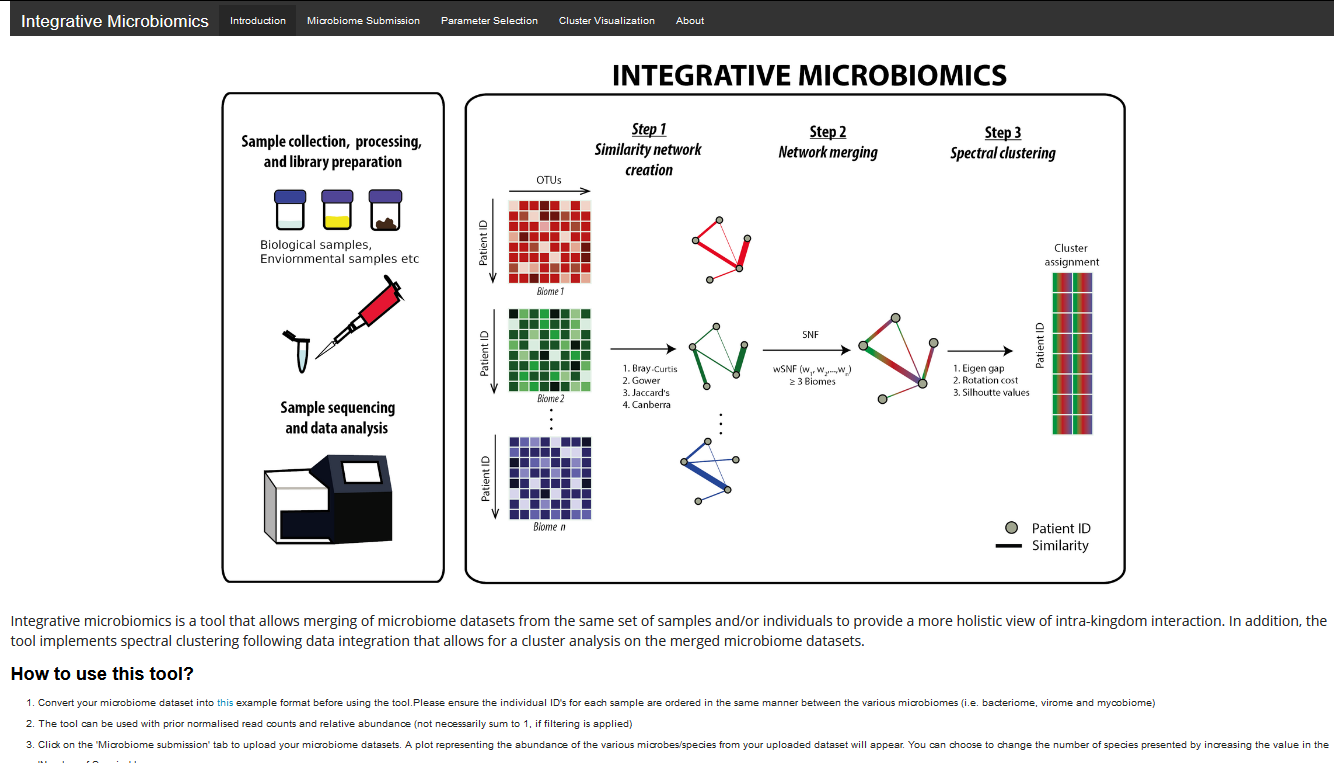
\includegraphics[width=0.8\textwidth]{image/Introduction_tab.PNG}
\end{figure}
This tab serves as the landing page of the web tool, containing an illustration of the workflow and a section on how to use the webtool. This page also provides an example format (csv) for the users to input their microbiome datasets.
\subsubsection{Microbiome submission tab}
\begin{figure}[!h]
	\centering
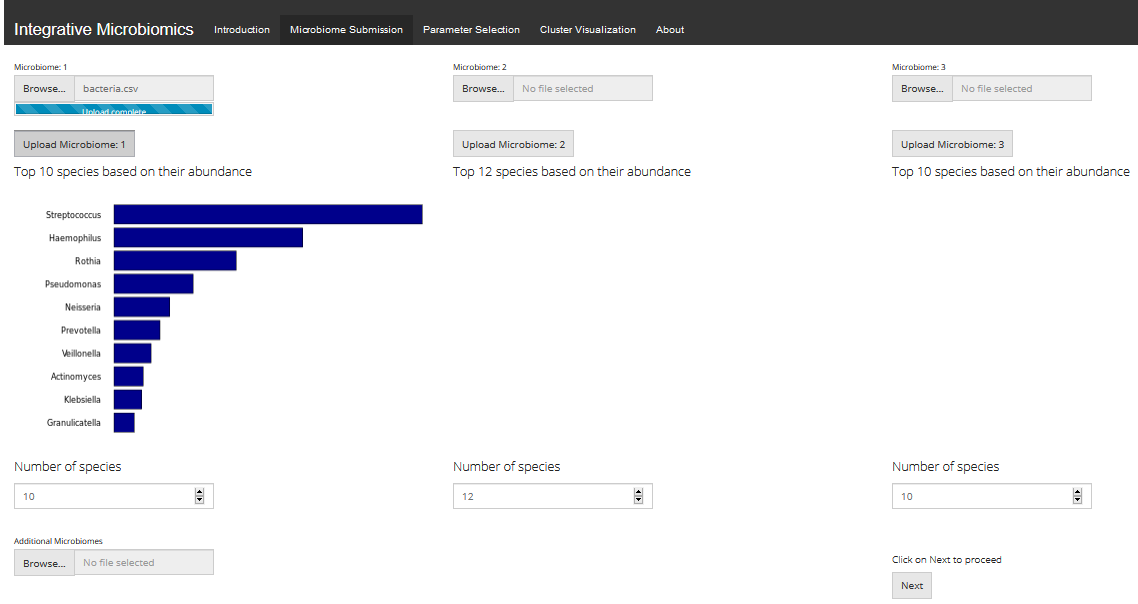
\includegraphics[width=0.8\textwidth]{image/microbiome_sub-tab.PNG}
\end{figure}
This page enables users to upload microbiome datasets, which they intend to integrate. The tool produces an abundance plot of top 10 microbes (can be modified by a scroll bar) if the microbiomes are successfully uploaded. Users who wish to integrate more than three microbiome datasets can use, the additional microbiomes option to upload any number of microbiome datasets. Maximum file size of up to 30MB is accepted for each microbiome dataset.
\subsubsection{Parameter selection tab}
\begin{figure}[H]
	\centering
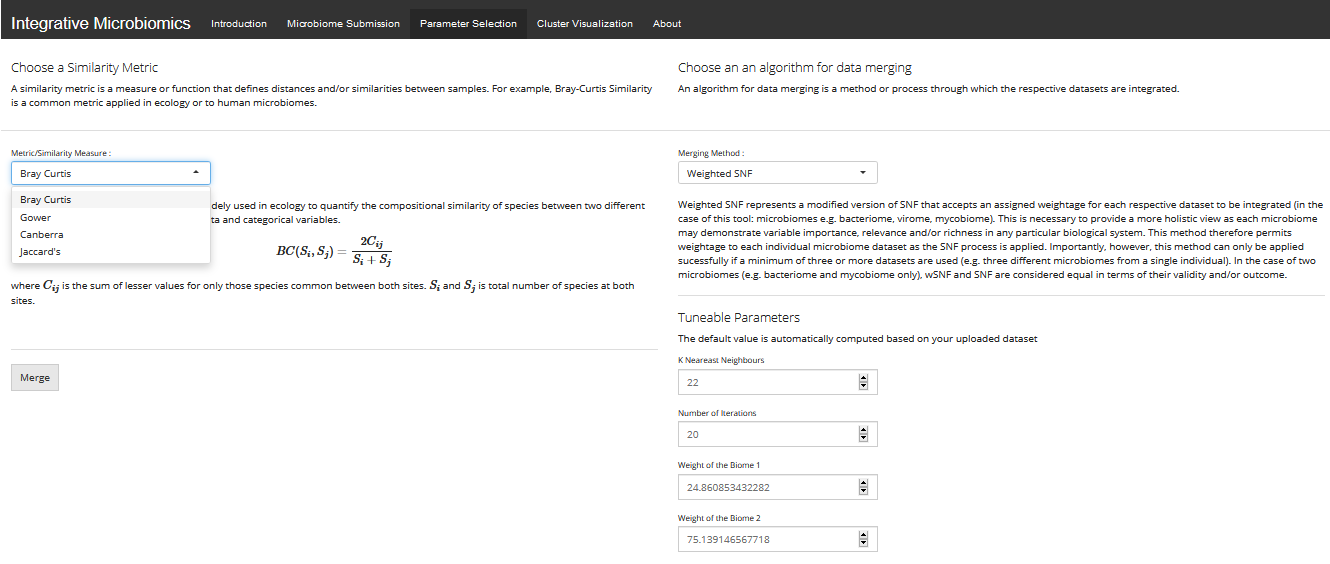
\includegraphics[width=0.8\textwidth]{image/parameter_sel-tab.png}
\end{figure}
This tab allows the users to select the merging algorithm 1)SNF or 2)Weighted SNF and a similarity measure. It also provides an option to set the model hyper-parameters of the merging algorithm such as number of iterations, the weights and the value of “k” nearest neighbours. The default values of these hyper parameters are set based on the input dataset.
\subsubsection{Cluster visualization tab}
\begin{figure}[H]
	\centering
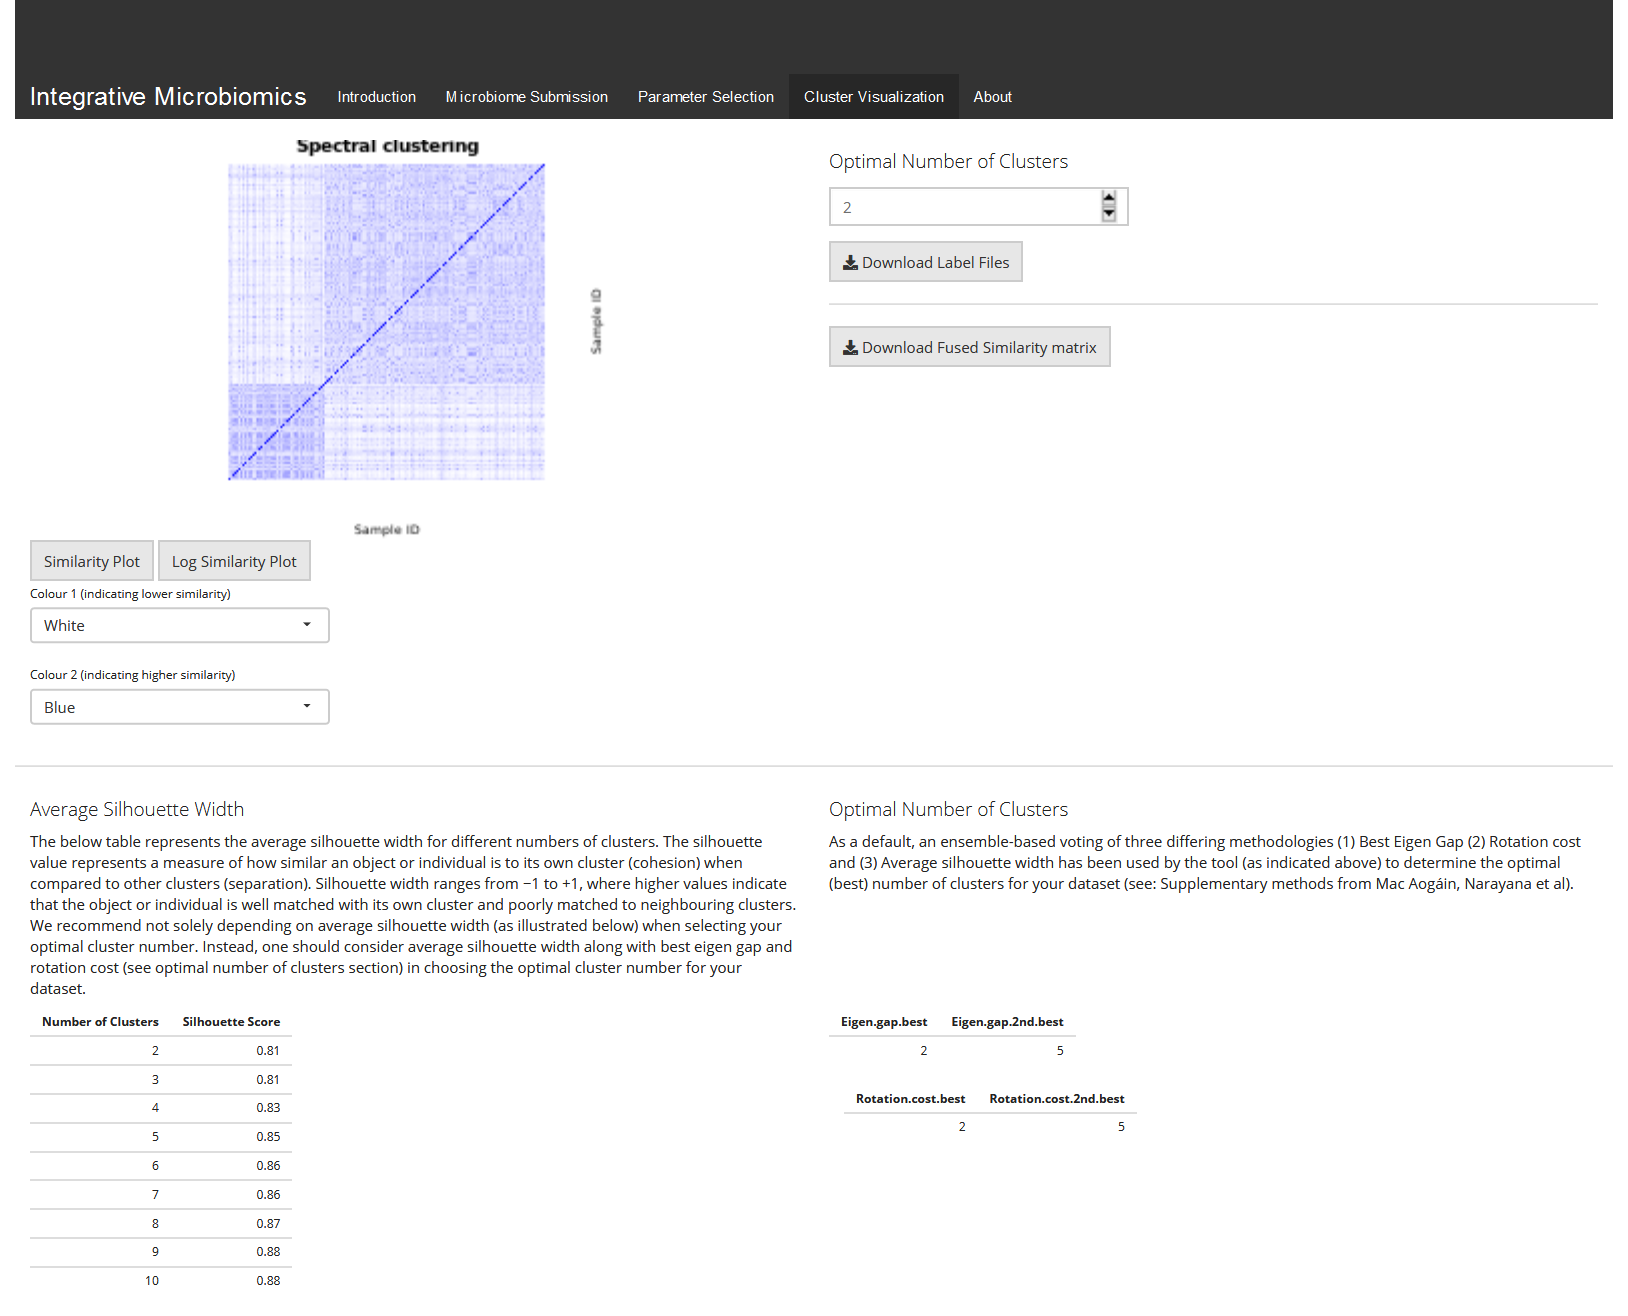
\includegraphics[width=0.8\textwidth]{image/cluster_vis-tab.png}
\end{figure}
This tab allows the users to visualize; the user-specified optimum number of clusters, as a heatmap of the patient/sample similarity matrix. The default value for optimum number of clusters is calculated based on ensemble-based voting of three differing methodologies as described in the methods. Further, this page also outputs the results from the three methodologies to aid the users to  select the optimum number of clusters. Additionally, this page provides option for users to download the cluster memberships of samples/patients (as csv) and the integrated patient/sample similarity matrix (as csv).
\subsubsection{About tab}
\begin{figure}[H]
	\centering
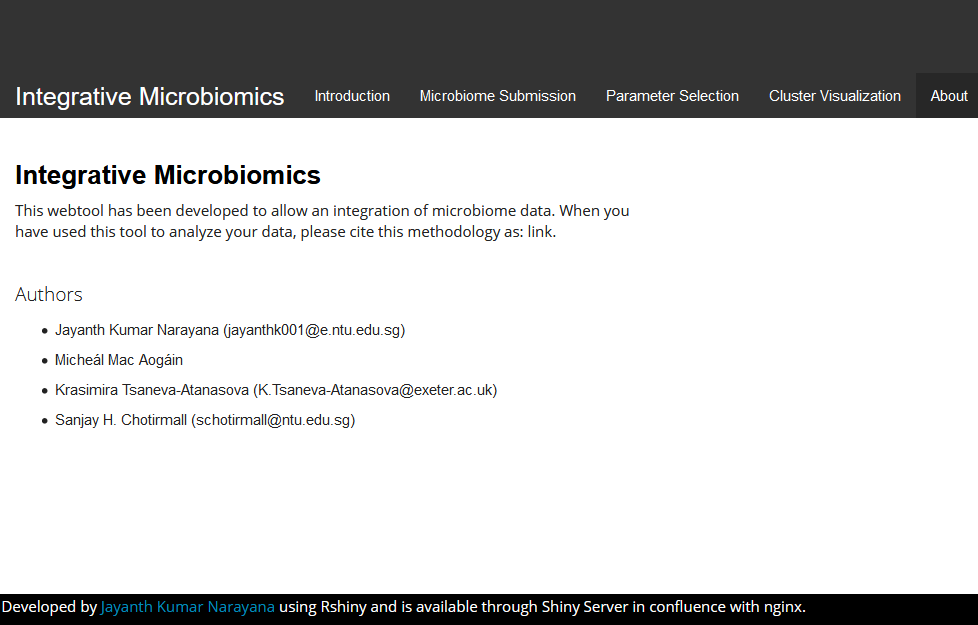
\includegraphics[width=0.8\textwidth]{image/about-tab.png}
\end{figure}
This page provides the link to the article, which the users could cite if they had used the tool. This page also provides a list of authors and their contacts, to report any concerns and feedback.

\subsection{``Integrative Microbiomics" identifies biologically relevant clusters}

To evaluate the added advantage of integrating datasets over singular analysis, and superiority of Integrative Microbiomics over conventional concatenation we performed an unsupervised clustering on three datasets (two publicly available datasets and CAMEB derivation/example dataset). We then evaluated the clusters on the available meta-data. Clustering of the individual biomes and the concatenated biomes were performed using spectral clustering and cluster comparisons using a chi-squared or Kruskal-Wallis test wherever applicable. The cluster consistency was assessed using Average Silhouette score. Assessing the results from the three examples (Table \ref{tab1}, \ref{tab2} and 3) shows an increased cluster consistency for the clusters derived using integrative microbiomics. Additionally, we observe an increased precision in identifying meaningful clusters, reflected by the decrease in the p-value for the evaluation of the features/meta-data between the clusters.\\

\subsubsection{Example 1: Oral Lichen Planus(OLP) dataset}
All paired-end fastq files containing ITS2 and 16S rRNA sequences and the accompanying meta-data of the saliva samples under accession number SRP067603 were retrieved from NCBI SRA as described in \cite{Li2019}. Pre-processing (filtering, trimming, de-replication, merging paired reads, removal of primers and chimeras) and taxonomy profiling (using UNITE 02.02.2019 release for ITS2 and Silva version 132 for 16S rRNA) were carried out using DADA2 package. The resulting datasets of 52 samples were integrated using integrative microbiomics webtool with k=6 and method=”SNF”.\\

\begin{table}[H]
	\begin{tabular}{|l|l|l|l|l|}
		\hline
		& \textbf{Bacteria} & \textbf{Fungi} & \textbf{Concatenated} & \textbf{IM} \\ \hline
		\textbf{Number of Clusters}                      & 3                 & 3              & 2                     & 5                                 \\ \hline
		\textbf{Silhouette}                              & 0.28              & 0.69           & 0.326                 & 0.85                              \\ \hline
		\textbf{Class: Healthy or Erosion or Reticulate} & NS                & 0.025          & NS                    & 0.0385                            \\ \hline
		\textbf{IL17}                                    & NS                & NS             & NS                    & 0.002                             \\ \hline
		\textbf{IL23}                                    & NS                & NS             & NS                    & 0.03                              \\ \hline
		\textbf{Age}                                     & 0.033             & NS             & NS                    & NS                                \\ \hline
	\end{tabular}
	\caption{A table representing the optimal clusters derived from various views of the dataset using Spectral clustering with Bray-Curtis similarity and p-value for the assessment of meta-data on the derived clusters, computed using chiq-squared test or kruskal-wallis test, wherever appropriate. The optimal number of clusters was calculated using the eigen gap method; followed by an assessment of cluster consistency (Average silhouette width).  NS- Non-significant (p-value $>$ 0.05). IM: Integrative Microbiomics}
	\label{tab1}
\end{table}

\subsubsection{Example 2: Ecological (Soil) dataset}
Bacterial and Fungal OTU table described in \cite{Wagg2019} along with their meta-data was downloaded from the supplementary materials. These datasets on 48 samples were then integrated using integrative Microbiomics webtool with k=3 and method=”SNF”.\\

\begin{table}[H]
	\begin{tabular}{|l|l|l|l|l|}
		\hline
		& \textbf{Bacteria} & \textbf{Fungi} & \textbf{Concatenated} & \textbf{Integrative Microbiomics} \\ \hline
		\textbf{No. of clusters} & 2                 & 2              & 2                     & 2                                 \\ \hline
		\textbf{Silhouette}      & 0.44              & 0.645          & 0.51                  & 0.92                              \\ \hline
		\textbf{Block}           & NS                & NS             & NS                    & NS                                \\ \hline
		\textbf{Treatment}       & 0.0005            & 0.0005         & 0.0005                & 0.0005                            \\ \hline
		\textbf{Decom}           & 5.745e-07         & 1.863e-06      & 6.784e-07             & 5.942e-07                         \\ \hline
		\textbf{N2O}             & 0.03185           & 0.04419        & 0.02942               & 0.01801                           \\ \hline
		\textbf{grNt}            & 3.455e-05         & 0.0002598      & 2.131e-06             & 1.093e-06                         \\ \hline
		\textbf{herbNt}          & 0.0001019         & 0.0004297      & 1.331e-05             & 4.315e-08                         \\ \hline
		\textbf{legNt}           & 0.002282          & 0.004783       & 0.0001821             & 1.106e-05                         \\ \hline
		\textbf{grPt}            & 9.889e-06         & 5.978e-06      & 6.784e-07             & 5.563e-05                         \\ \hline
		\textbf{herbPt}          & 3.822e-05         & 0.0005955      & 7.879e-06             & 2.567e-09                         \\ \hline
		\textbf{legPt}           & 0.0006874         & 0.003719       & 0.0001038             & 4.614e-06                         \\ \hline
		\textbf{Pleach}          & 0.01              & 0.008947       & 0.002958              & 0.00924                           \\ \hline
		\textbf{Nleach}          & 0.003096          & 0.0001295      & 0.001887              & 0.002256                          \\ \hline
		\textbf{aveMF}           & 0.001669          & 0.0257         & 0.002037              & 9.519e-05                         \\ \hline
		\textbf{pcaMF}           & 5.744e-06         & 6.273e-05      & 6.784e-07             & 9.731e-10                         \\ \hline
	\end{tabular}
	\caption{A table illustrating the optimal clusters derived from various views of the dataset using Spectral clustering with Bray-Curtis similarity and p-values for the evaluation of meta-data using chiq-squared test or kruskal-wallis test, wherever appropriate are reported. The optimal number of clusters was calculated using the eigen gap method; followed by an assessment of cluster consistency (Average silhouette width). NS- Non-significant (p-value $<$ 0.05)}
	\label{tab2}
\end{table}

\subsubsection{Example 3: CAMEB dataset}
Microbiome, mycobiome and virome were derived from 217 patients of the CAMEB cohort \cite{Mac1800766}. This dataset was used as the example dataset to derive and evaluate Integrative Microbiomics. These datasets were integrated using integrative microbiomics webtool with k=8, method=`` Weighted SNF” and other parameters were set to default values.

\begin{figure}[H]
	\centering
	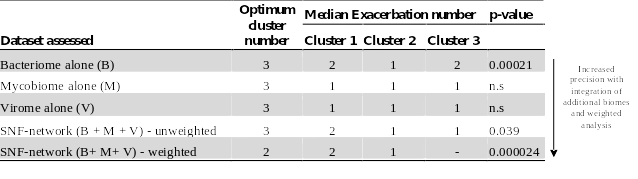
\includegraphics[width=0.8\textwidth]{image/table.png}
	\caption*{Table 3: A table illustrating the optimal clusters derived from various views of the dataset using Spectral clustering with Bray-Curtis similarity and p-values for the evaluation of meta-data using kruskal-wallis test are reported. The optimal number of clusters was calculated using the eigen gap method. NS- Non-significant (p-value $<$ 0.05)}
\end{figure}

\subsection{Increased antagonistic interaction during exacerbation with no difference in microbial diversity, $\alpha$ and $\beta$ diversity}

\begin{figure}[!htb]
	\centering
	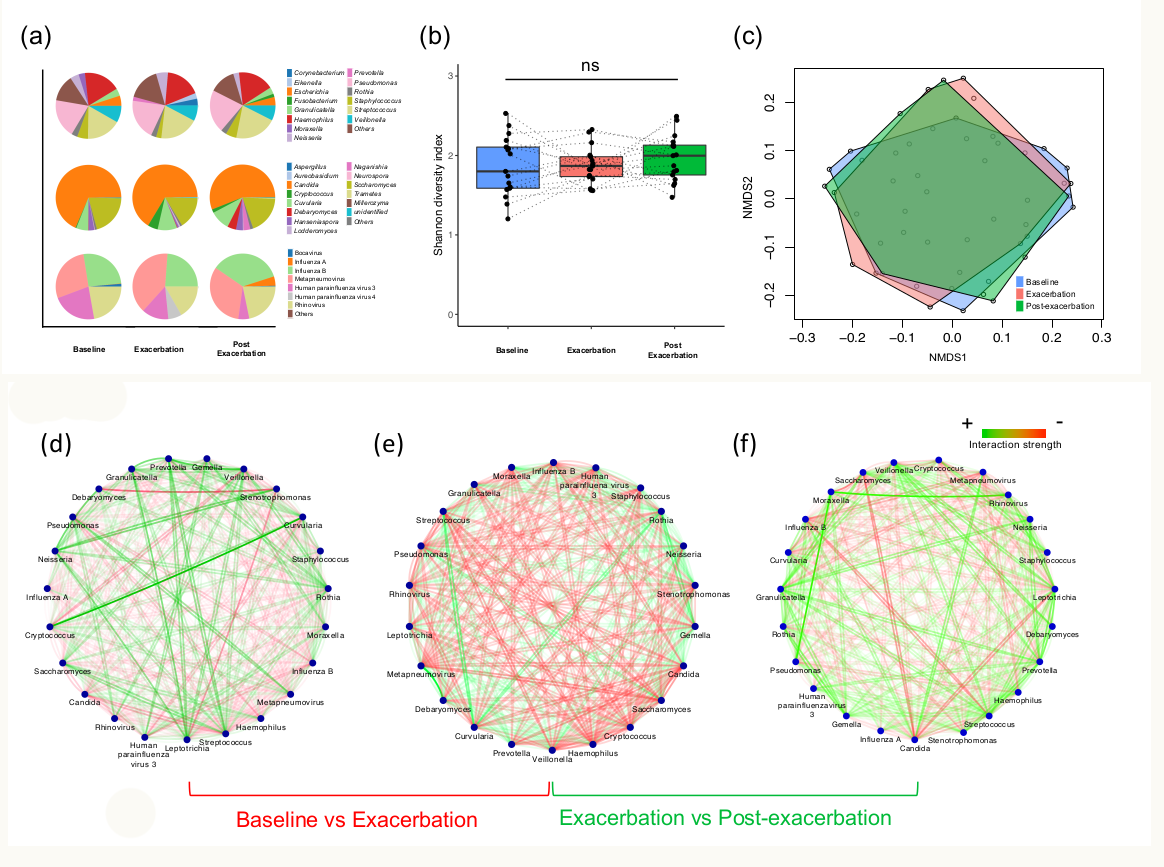
\includegraphics[width=\textwidth]{image/longitudinal.png}
	\caption{Longitudinal analysis of the integrated multi-biome during bronchiectasis exacerbations. (a) Bacterial, fungal and viral community status were assessed longitudinally in n=17 bronchiectasis patients at baseline (pre-exacerbation) (‘B’), during an established pulmonary exacerbation (‘E’) and then post-exacerbation (‘P’) following completion of antibiotic therapy. Pie charts illustrate aggregate microbial composition of the bacterial, fungal and viral community profiles across each time point with the most abundant taxa indicated by the colour legend. (b) Boxplots illustrating comparable $\alpha$-diversity across baseline (‘B’), exacerbation (‘E’) and post-exacerbation (‘P’) specimens. Dotted lines indicate the longitudinal pattern of each individual patient (n=17). (c) Non-metric Multi-Dimensional Scaling (NMDS) plot illustrating comparable multi-biome $\beta$-diversity across baseline (‘B’), exacerbation (‘E’) and post-exacerbation (‘P’) specimens. Samples are grouped according to their respective longitudinal timepoint. (d-f) Visualization of the interactome’s positive and negative interactions between the most abundant taxa at (d) baseline (pre-exacerbation), (e) during exacerbation and (f) post-exacerbation. Interactions between microbes are classified as negative if the sign of the edge weights between them is negative (coloured red) with positive interactions indicated by green colouration.}
	\label{fig4}
\end{figure}

Next, to study exacerbation events using the interactome framework; we assessed the interactome at baseline (pre-exacerbation), during exacerbation and post-exacerbation. A comparison of the longitudinal multi-biome signatures across time points revealed no significant difference in microbial composition (Fig \ref{fig4} a), $\alpha$ (Fig \ref{fig4} b) and $\beta$ (Figure \ref{fig4} c) diversity suggesting overall stability of the microbiome during exacerbation. On the contrary, co-occurrence analysis reveals significant changes in the interactome with an increased number and strength of negative interactions during exacerbation as opposed to baseline and post exacerbation. In-depth analysis of changes in the interactome from baseline to post-exacerbation state reveals a reduced number of total interactions in the post-exacerbation state, likely explained by the broad antibiotics usage, which eliminates potential interacting microbes.\\

\subsection{Simulation of the antibiotic action using the Interactome framework reliably predicts the rank order difference of key microbial taxa}

\begin{figure}[!htb]
	\centering
	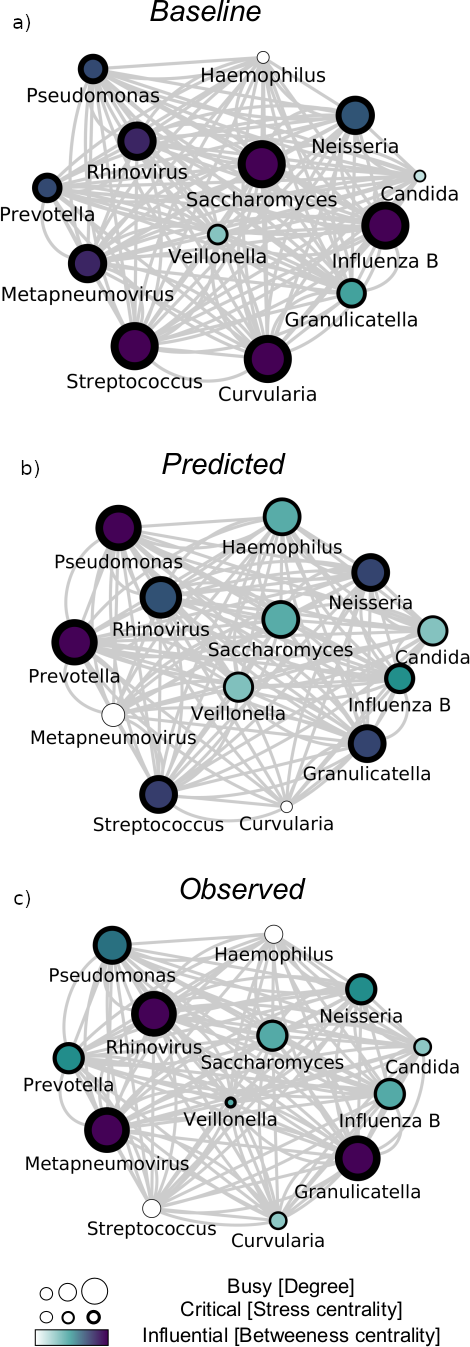
\includegraphics[width=0.4\textwidth]{image/antibiotic.png}
	\caption{(a) Baseline network analysis of bronchiectasis patients who subsequently received $\beta$-lactam therapy for treatment of an exacerbation (n=12). (b) a simulated network based on 75\% reduction in the abundance of $\beta$-lactam-susceptible organisms and calculation of the re-configured network. (c) observed network reconfiguration in patients following $\beta$-lactam therapy. Circle size, outline thickness and colour respectively represent node importance based on network metrics; degree, stress centrality and betweenness centrality}
	\label{fig5}
\end{figure}

To evaluate the clinical utility of our derived network-based interactomes by predicting the influence of antibiotic exposure on its contained microbiome. As several (n=12) patients of our longitudinal cohort received -lactam antibiotics for treatment of their initial exacerbation, we used the baseline (pre-$\beta$-lactam exposure) interactome network (Figure \ref{fig5}a) to predict network reconfiguration post $\beta$-lactam treatment by artificially reducing the abundance of $\beta$-lactam-sensitive microbes by 75\% (Figure \ref{fig5}b). We then compared our ‘simulated’ network to that observed among our $\beta$-lactam-treated patients following therapy (Figure \ref{fig5}c). Our network-based prediction had reliable comparability to the network observed in $\beta$-lactam-treated patients with respect to several microbial nodes. Notably, the rank order difference in key microbial taxa post-antibiotic treatment was correctly predicted for 10 out of 13 taxa in our simulated model.\\

\subsection{wSNF and Interactome analysis on the validation cohort rediscovers a ``high-risk" cluster and validates the interactome.}

To assess and validate the previously derived “high-risk” cluster, we reimplemented the weighted Similarity Network Fusion (wSNF) followed by spectral clustering on the multi-biome derived from a validation cohort (n=166) using a metagenomic sequencing approach, contrary to the targeted sequencing approach used previously. Integrative Microbiomics identified two clusters, with one exhibiting an increased exacerbation phenotype. Thus, validating the “high-risk” cluster of bronchiectasis patients (Figure \ref{fig6}a). Furthermore, Interactome analysis of the “high-risk” cluster derived from the validation cohort identifies 89.9\% of the interactions from the derivation cohort (Figure \ref{fig6}b). Hence, validating the interactome signature of the “high-risk” cluster.

To further assess and validate specific interactions within our derived interactomes, we selected the interaction between P. aeruginosa and A. fumigatus for further interrogation since, it is known that they frequently co-exist in the airway of respiratory disease patients (Cystic Fibrosis and Bronchiectasis). Furthermore, it has been shown that they can inhibit \cite{Ferreira2015,Reece2018} or promote \cite{Briard2016,Margalit2020} each other’s growth. These two organisms exhibit opposing interactions from our originally derived clusters (Figure \ref{fig7}a): co-exclusion in the low and co-occurrence in the high exacerbation frequency clusters respectively (Figure \ref{fig7}a). Comparisons of P. aeruginosa clinical isolates derived from patients belonging to the low and high exacerbation frequency clusters reveal these contrasting interactions (Figure \ref{fig7}b). Consistent with the observation from our derived interactomes, the low exacerbation frequency cluster isolate (LEF) exhibited negative interactions with A. fumigatus whereas no such inhibitory effect was observed with the high exacerbation frequency cluster isolate (HEF) (Figure \ref{fig7}c). Further analysis of pyoverdine levels reveals a hyperproduction in the HEF isolate exceeding that of the LEF or the PAO1 control. As pyoverdine demonstrates anti-A. fumigatus properties and allows P. aeruginosa to coexist, these findings offer a potential mechanism for our in-vitro observations which most critically are consistent with our in vivo-derived interactomes further validating their accuracy and clinical relevance.\\

\begin{figure}[!htb]
	\centering
	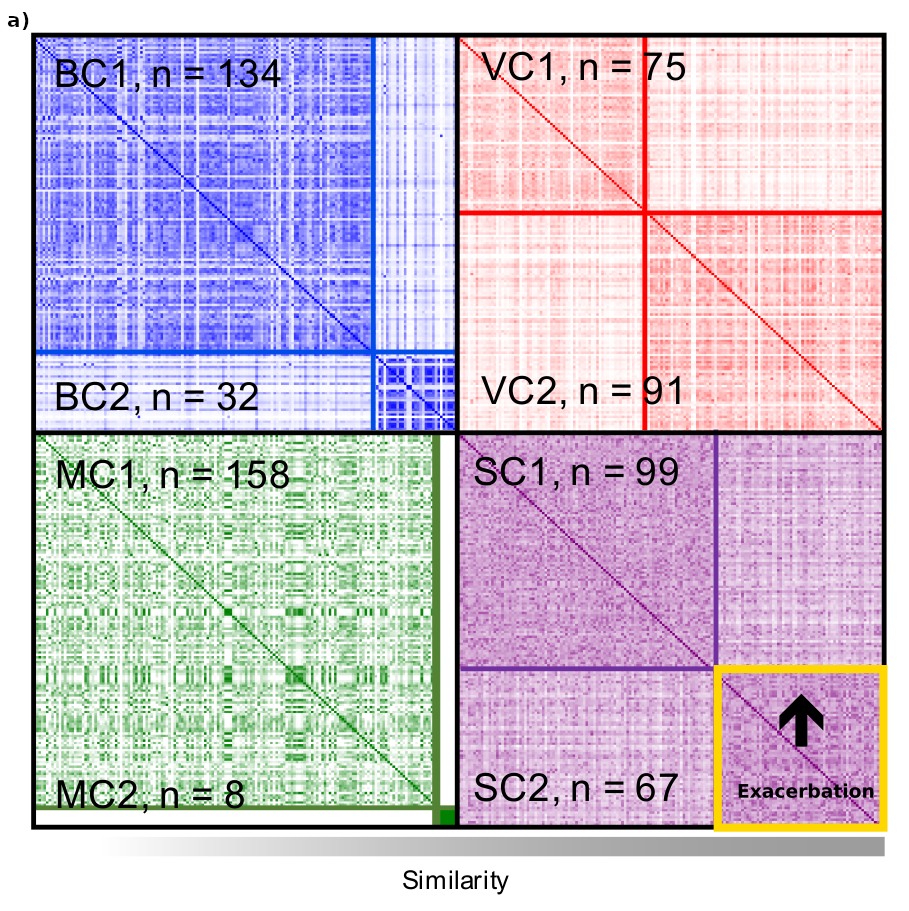
\includegraphics[width=0.5\textwidth]{image/meta_validation1.png}
	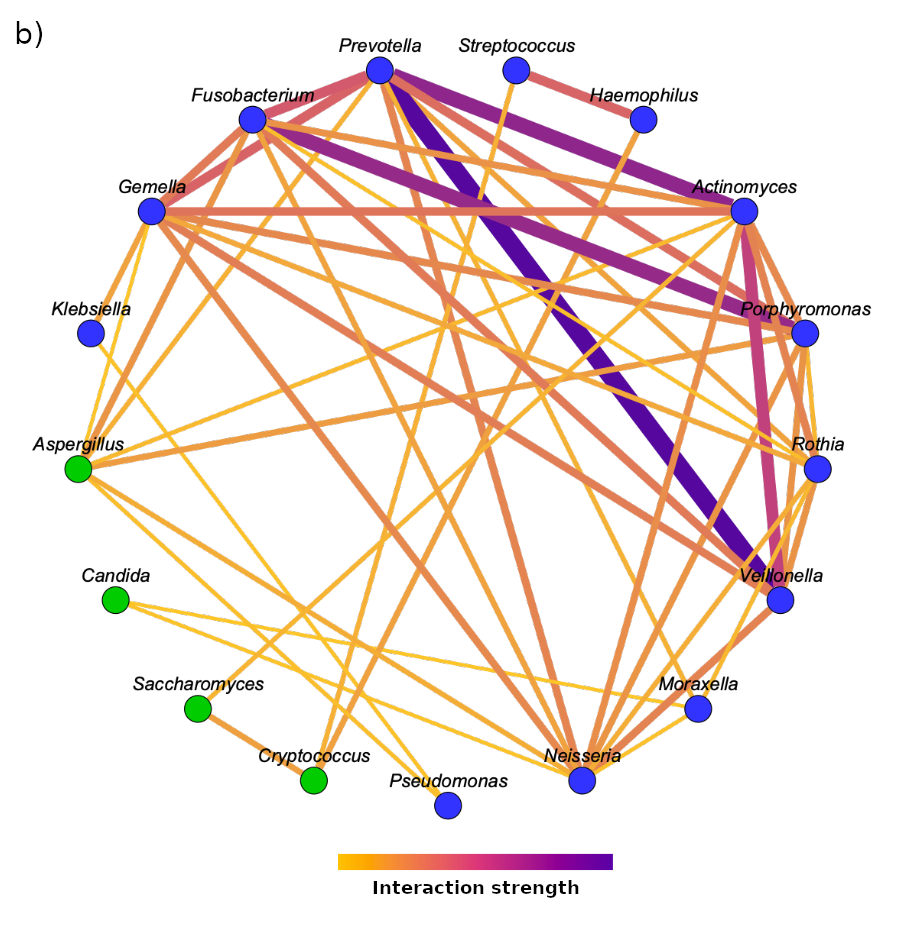
\includegraphics[width=0.5\textwidth]{image/meta_validation2.png}
	\caption{(a) Metagenomic integration of microbiomes: A patient similarity matrix illustrating patient clusters derived using spectral clustering of Microbiome (BC), Mycobiome (MC),Virome (VC) and SNF integrated (SC) patient similarity matrices, (b)Interactome signature of the “high-risk” cluster: an interactome plot with nodes as microbes (common between “high-risk” cluster of the derivation and validation cohort) and edges as interactions. Node colour indicates bacteria (blue) and fungi (green). Edge width and colour represent the interaction strength. }
	\label{fig6}
\end{figure}


\begin{figure}[!htb]
	\centering
	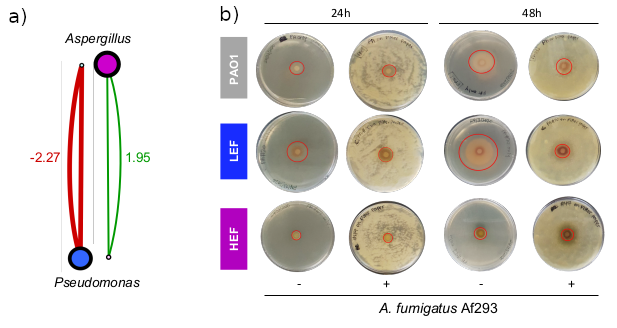
\includegraphics[width=0.5\textwidth]{image/exp_validation1.png}%
	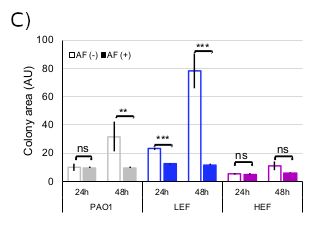
\includegraphics[width=0.4\textwidth]{image/exp_validation2.png}
	\caption{(a) Node and edge plots extracted from the LEF and HEF network cluster analysis highlighting opposing interactions between P. aeruginosa and A. fumigatus related to exacerbation frequency. Edges are coloured green or red, reflecting a positive (co-occurrence) or negative (co-exclusion) interaction, respectively. Circle size, outline thickness and colour respectively represent node importance based on network metrics; degree, stress centrality, and betweenness centrality. (b) Demonstration of strain-dependent inter-kingdom interaction between P. aeruginosa and A. fumigatus. Comparison of direct interactions between P. aeruginosa laboratory strain (‘PAO1’; grey) and isolates obtained from patients from the LEF and HEF clusters respectively (‘LEF’; blue, ‘HEF’; purple) with A. fumigatus (Af293) by disk inhibition assays. Colony zone diameter is indicated by a red circle for P. aeruginosa strains grown in the presence (+) or absence of (-) Af293 at 24h and 48h timepoints, respectively. (c) Analysis of P. aeruginosa zone diameters observed following co-culture with Af293 following 24h and 48h incubation. Bars are coloured according to the respective P. aeruginosa strain as described above. Open bars indicate zone diameters observed in the absence of A. fumigatus and filled bars indicate zone diameters observed on co-culture. Error bars represent the standard deviation of triplicate determinations. ns: non-significant; **p$<$0.01; ***p$<$0.001.}
	\label{fig7}
\end{figure}

\subsection{Interactions better predict time to next exacerbation over individual taxa.}

To assess, the clinical applicability of the interactome framework we tried to assess the predictability of “Time to next exacerbation” given the post-exacerbation microbiome by considering individual taxa and interactions (pairs of microbes) as features. A correlation analysis revealed that a greater number of pairwise interactions compared to individual taxa are correlated with “Time to next exacerbation” (Figure \ref{fig8}ab) irrespective of the time point (Baseline, Exacerbation and Post-exacerbation). Evaluation of the accuracy of the Non-linear prediction model fitted to predict “Time to next exacerbation” reveals that the post-exacerbation microbiome is a better predictive than the baseline and exacerbation microbiomes. Additionally, there is a major increase of predictive capacity (Figure \ref{fig8}c) (0.551 $>$ 0.239) if interactions are used as features as opposed to individual taxa; suggesting that pairwise interaction of microbes are better markers to study and associate disease outcomes.  


\begin{figure}[!htb]
	\centering
	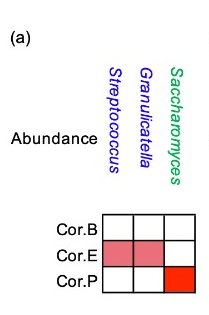
\includegraphics[width=0.15\textwidth]{image/1.jpeg}%
	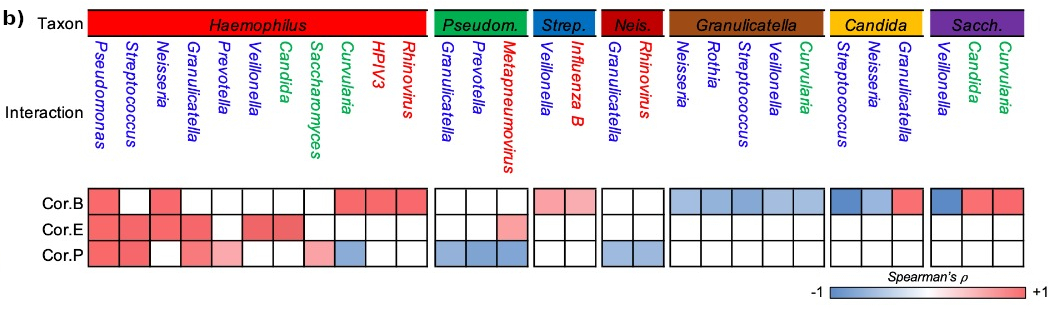
\includegraphics[width=0.75\textwidth]{image/3.jpeg}
	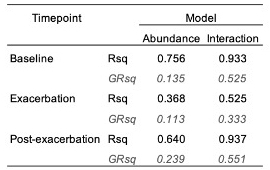
\includegraphics[width=0.5\textwidth]{image/5.jpeg}
	\caption{A correlogram illustrating the individual taxa (a) and pairwise interactions (b) significantly correlated with time to next exacerbation at various time points: Baseline (Cor.B), Exacerbation (Cor.E) and Post-exacerbation (Cor.P). (c) A table illustrating the evaluation metrics of the MARS, a non-linear regression model when fitted to predict time to next exacerbation using individual taxa abundance and pairwise interaction strength as predictors/features.}
	\label{fig8}
\end{figure}